\section{Appendix} \label{sec:appendix}

\begin{figure}
  \begin{center}
    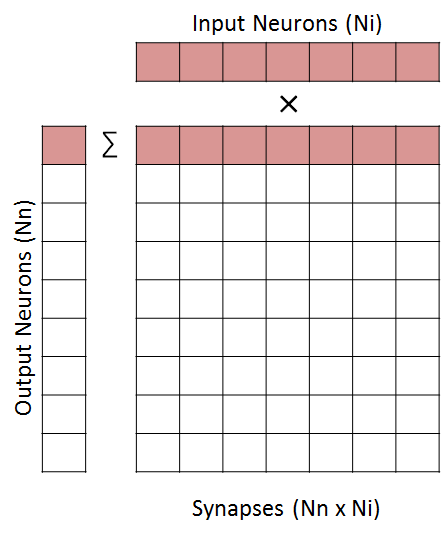
\includegraphics[width=\linewidth]{cs758-figs/classifier-diagram.png}
  \end{center}
\vspace{-0.2in}
  \caption{Classifier workload diagram}
  \label{fig:classifier-diagram}
\vspace{-0.05in}
\end{figure}

Figure~\ref{fig:classifier-diagram} shows the classifier workload. 
Classifier requires multiplying the input neurons (a vector) by synapses 
(a matrix) and then doing the summation reduction.


\begin{figure}
  \begin{center}
    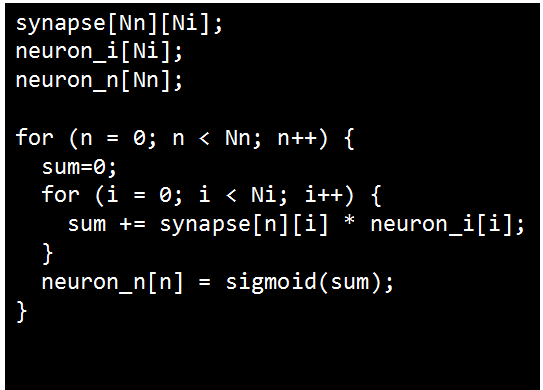
\includegraphics[width=\linewidth]{cs758-figs/classifier-cpu.png}
  \end{center}
\vspace{-0.2in}
  \caption{Classifier implementation using sequential cpu}
  \label{fig:classifier-cpu}
\vspace{-0.05in}
\end{figure}

Figure~\ref{fig:classifier-cpu} shows the sequential implementation of 
classifier. Classifier can be done with a nested for loop to take the 
summation of the product between the input neurons and synapses.


\begin{figure}
  \begin{center}
    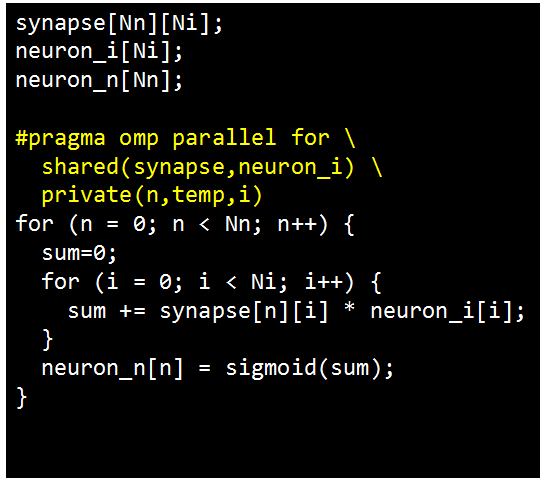
\includegraphics[width=\linewidth]{cs758-figs/classifier-omp.png}
  \end{center}
\vspace{-0.2in}
  \caption{Classifier implementation using OpenMP}
  \label{fig:classifier-omp}
\vspace{-0.05in}
\end{figure}

Figure~\ref{fig:classifier-omp} shows the OpenMP implementation of 
classifier. The OpenMP implementation of classifier is using a 
"#pragma omp parallel for" on the outer loop. 


\begin{figure}
  \begin{center}
    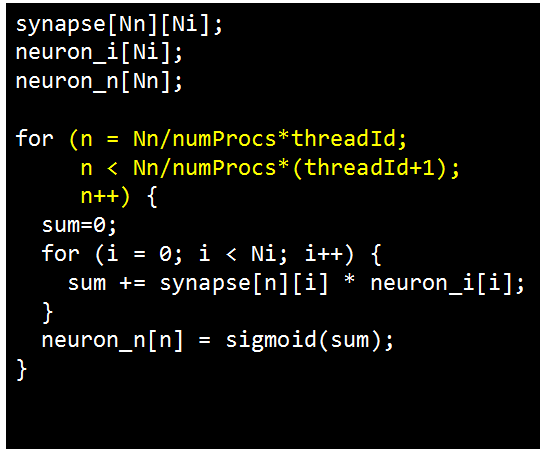
\includegraphics[width=\linewidth]{cs758-figs/classifier-pthread.png}
  \end{center}
\vspace{-0.2in}
  \caption{Classifier implementation using pthreads}
  \label{fig:classifier-pthread}
\vspace{-0.05in}
\end{figure}

Figure~\ref{fig:classifier-pthread} shows the pthread implementation of 
classifier. The pthreads implementation of classifier shards the 
workload among pthreads. 


\begin{figure}
  \begin{center}
    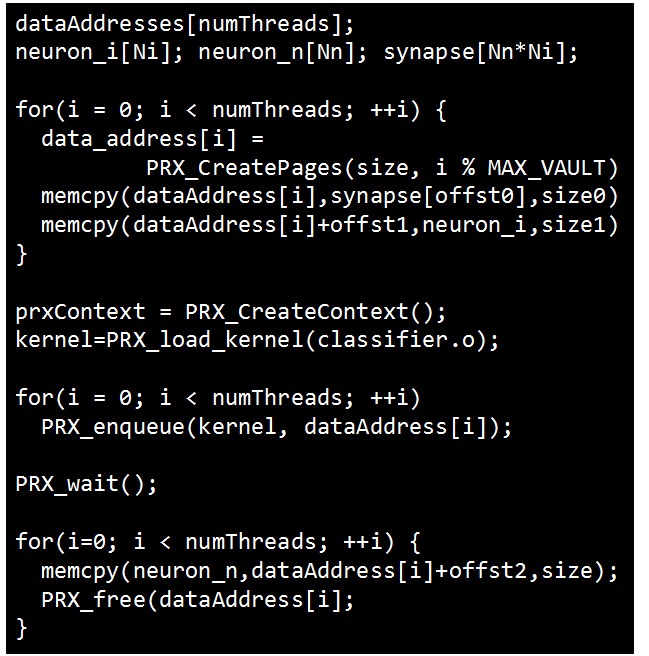
\includegraphics[width=\linewidth]{cs758-figs/classifier-prx_inorder_q.png}
  \end{center}
\vspace{-0.2in}
  \caption{Classifier implementation using proximate with inorder cores and queuing model}
  \label{fig:classifier-prx_inorder_q}
\vspace{-0.05in}
\end{figure}

Figure~\ref{fig:classifier-prx_inorder_q} shows the proixmate implementation 
with inorder cores and queuing model of classifier. The proximate queueing implementation of classifier shards the 
workload to different vaults. Calling create context 
will spawn threads to monitor work queues. Then, load the kernel so that each thread
know which kernel to execute. Next, enqueue the workloads and wait for them to finish. 
Finally, gather the results back into a single array. 


\begin{figure}
  \begin{center}
    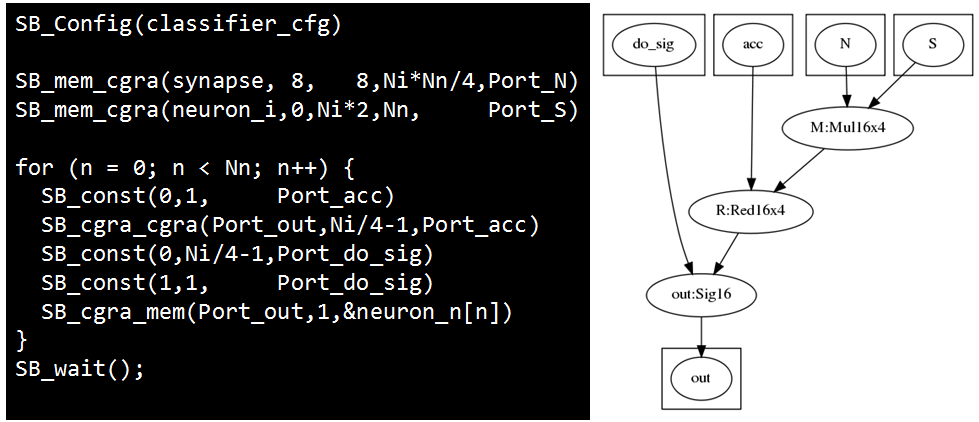
\includegraphics[width=\linewidth]{cs758-figs/classifier-prx_sb_only.png}
  \end{center}
\vspace{-0.2in}
  \caption{Classifier implementation using proximate with softbrain only}
  \label{fig:classifier-prx_sb_only}
\vspace{-0.05in}
\end{figure}

Figure~\ref{fig:classifier-prx_sb_only} shows the proixmate implementation 
with softbrain only of classifier. Classifier can be parallelized 
using proximate with queueing by first sharding the workload. Calling create context 
will spawn threads to monitor work queues. Then, load the kernel so that each thread
know which kernel to execute. Next, enqueue the workloads and wait for them to finish. 
Finally, gather the results back into a single array. 
shows speedups relative to a single 
thread of image processing convolution engine applications using OpenMP on Xeon 
Phi. Note that DoG omp outperforms pthreads, probably because of dynamic 
scheduling. Therefore, comparing proximate to both pthreads and OpenMP is 
important for performance evaluation. 
